\documentclass{../../../oss-classkick-exam}
\usepackage{bm}

\begin{document}
\genheader

\gentitle{C}{DYNAMICS}

\genmultidirections

\gengravity

\raggedcolumns
\begin{multicols*}{2}
  \textbf{Questions \ref{q:2blocks1}--\ref{q:2blocks2}}\\
  Two blocks, \SI{4}{\kilo\gram} and \SI{2}{\kilo\gram}, are connected by a
  string. An applied force $F$ of magnitude \SI{18}{\newton} pulls the blocks
  to the left.
  \begin{center}
    \begin{tikzpicture}[scale=.95]
      \fill[pattern=north east lines] (2.5,0) rectangle(9,-.3);
      \begin{scope}[thick]
        \draw (2.5,0)--(9,0);
        \draw (7,0) rectangle(8,1) node[midway]{2 kg};
        \draw (4,0) rectangle(6,1) node[midway]{4 kg};
        \draw (6,.5)--(7,.5);
        \draw[->] (4,.5)--(3,.5) node[midway,above]{\SI{18}{\newton}};
      \end{scope}
    \end{tikzpicture}
  \end{center}

  \begin{questions}
    \question The acceleration of the \SI{4}{\kilo\gram} block is
    \begin{choices}
      \choice\SI2{\metre\per\second\squared}
      \choice\SI3{\metre\per\second\squared}
      \choice\SI4{\metre\per\second\squared}
      \choice\SI{4.5}{\metre\per\second\squared}
      \choice\SI6{\metre\per\second\squared}
    \end{choices}
    \label{q:2blocks1}
    
    \question The tension in the string between the blocks is
    \begin{choices}
      \choice 4 N
      \choice 6 N
      \choice 12 N
      \choice 16 N
      \choice 18 N
    \end{choices}
    \label{q:2blocks2}

    \fullwidth{
      \textbf{Questions \ref{pos1}--\ref{pos2}}\\
      The position of a \SI{2}{\kilo\gram} object is described by the equation
      $x=2t^2-3t^3$, where $x$ is in meters and $t$ is in seconds.
    }

    \question The net force acting on the object at a time of \SI{1}{\second} is
    \begin{choices}
      \choice\SI{-4}\newton
      \choice\SI{-8}\newton
      \choice\SI{-14}\newton
      \choice\SI{-20}\newton
      \choice\SI{-28}\newton
    \end{choices}
    \label{pos1}
    
    \question The net force acting on the object is positive from $t=0$ until a
    time of
    \begin{choices}
      \choice\SI{.11}{\second}
      \choice\SI{.22}{\second}
      \choice\SI{.44}{\second}
      \choice\SI{.67}{\second}
      \choice\SI{1.}{\second}
    \end{choices}
    \label{pos2}

    \fullwidth{
      \textbf{Questions \ref{q:striaght1}--\ref{q:striaght2}}\\
      An object of mass $m$ moves along a straight line with a speed described
      by the equation $v=c+bt^3$.
    }

    \question The initial velocity of the mass is
    \begin{choices}
      \choice $c$
      \choice $ct+bt^3$
      \choice $ct+bt^4$
      \choice $bt^2$
      \choice $bt$
    \end{choices}
    \label{q:striaght1}

    \question The net force acting on the mass at time $T$ is
    \begin{choices}
      \choice $3mbT$
      \choice $3mbT^2$
      \choice $3mbT^3$
      \choice $mc+2mbT^2$
      \choice $mc^2+4mbT^4$
    \end{choices}
    \label{q:striaght2}
    \columnbreak

    \fullwidth{
      \textbf{Questions \ref{q:pulley1}--\ref{q:pulley2}}\\
      A system consists of two blocks having masses of \SI{2}{\kilo\gram} and
      \SI{1}{\kilo\gram}. The blocks are connected by a string of negligible
      mass and hung over a light pulley, and then released from rest.
      \begin{center}
        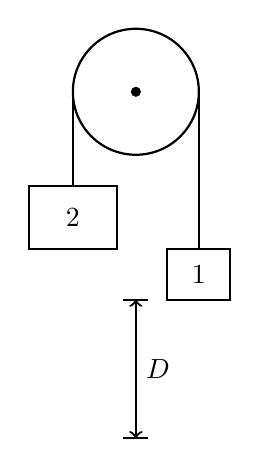
\begin{tikzpicture}[scale=.8]
          \begin{scope}[thick]
            \draw(0,0) circle(1);
            \fill(0,0) circle(.08);
            \draw(1,0)--(1,-2.5);
            \draw(.5,-2.5) rectangle(1.5,-3.3) node[midway]{\SI1{\kilo\gram}};
            \draw(-1,0)--(-1,-1.5);
            \draw(-1.7,-1.5) rectangle(-.3,-2.5) node[midway]{\SI2{\kilo\gram}};
            \draw(-.2,-3.3)--(.2,-3.3);
            \draw(-.2,-5.5)--(.2,-5.5);
            \draw[<->](0,-3.3)--(0,-5.5) node[midway,right]{$D$};
          \end{scope}
        \end{tikzpicture}
      \end{center}
    }

  \question The acceleration of the \SI{2}{\kilo\gram} block is most nearly
    \begin{choices}
      \choice $\displaystyle\frac{2}{9}g$
      \choice $\displaystyle\frac{1}{3}g$
      \choice $\displaystyle\frac{1}{2}g$
      \choice $\displaystyle\frac{2}{3}g$
      \choice $g$
    \end{choices}
    \label{q:pulley1}
    
    \question The speed of the \SI{2}{\kilo\gram} block after it has descended a
    distance $D$ is most nearly
    \begin{choices}
      \choice $\displaystyle\sqrt{\frac{4gD}{3}}$
      \choice $\displaystyle\sqrt{\frac{2gD}{3}}$
      \choice $\displaystyle\sqrt{\frac{gD}{3}}$
      \choice $\displaystyle\sqrt{\frac{gD}{2}}$
      \choice $\displaystyle\sqrt{\frac{4gD}{6}}$
    \end{choices}
    \label{q:pulley2}

    \fullwidth{
      \textbf{Questions \ref{3blks1}--\ref{3blks2}}\\
      Three blocks of mass \SI{3}{\kilo\gram}, \SI{2}{\kilo\gram}, and
      \SI{1}{\kilo\gram} are pushed along a horizontal frictionless plane by a
      force of \SI{24}{\newton} to the right, as shown.
      \begin{center}
        \begin{tikzpicture}[scale=.9]
          \fill[pattern=north east lines] (0,0) rectangle(8,-.3);
          \begin{scope}[thick]
            \draw (0,0)--(8,0);
            \draw (2,0) rectangle(4,1.5) node[midway]{3 kg};
            \draw (4,0) rectangle(5.5,1.3) node[midway]{2 kg};
            \draw (5.5,0) rectangle(6.5,1.1) node[midway]{1 kg};
            \draw[->](0,.75)--(2,.75) node[midway,above]{24 N};
          \end{scope}
        \end{tikzpicture}
      \end{center}
    }

    \question The acceleration of the \SI{2}{\kilo\gram} block is
    \begin{choices}
      \choice\SI{144}{\metre\per\second\squared}
      \choice\SI{72}{\metre\per\second\squared}
      \choice\SI{12}{\metre\per\second\squared}
      \choice\SI{6}{\metre\per\second\squared}
      \choice\SI{4}{\metre\per\second\squared}
    \end{choices}
    \label{3blks1}
    
    \question The force that the \SI{2}{\kilo\gram} block exerts on the
    \SI{1}{\kilo\gram} block is
    \begin{choices}
      \choice\SI{2}{\newton}
      \choice\SI{4}{\newton}
      \choice\SI{6}{\newton}
      \choice\SI{24}{\newton}
      \choice\SI{144}{\newton}
    \end{choices}
    \label{3blks2}
    \columnbreak

    \question A block of mass \SI{4}{\kilo\gram} slides down a rough incline
    with a constant speed. The angle the incline makes with the horizontal is
    \ang{30}. The coefficient of friction acting between the block and incline
    is most nearly
    \begin{center}
      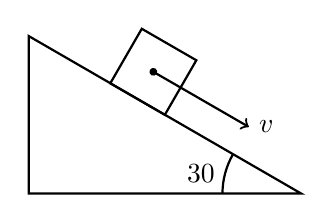
\begin{tikzpicture}
        \begin{scope}[thick]
          \draw(0,0)--(-3.46,0)--(-3.46,2)--cycle;
          \draw[thick](-1,0) arc(180:150:1) node[midway,left]{\ang{30}};
        \begin{scope}[rotate=-30]
          \draw(-2,0) rectangle(-2.8,.8);
          \fill(-2.4,.4) circle(.05);
          \draw[->](-2.4,.4)--(-1.,.4)node[right]{$v$};
        \end{scope}
      \end{scope}
      \end{tikzpicture}
    \end{center}
    \begin{choices}
      \choice 0.1
      \choice 0.2
      \choice 0.3
      \choice 0.4
      \choice 0.6
    \end{choices}

    \question A ball is thrown straight up into the air, encountering air
    resistance as it rises. What forces, if any, act on the ball as it rises?
    \begin{choices}
      \choice A decreasing gravitational force and an increasing force of air
      resistance
      \choice An increasing gravitational force and an increasing force of air
      resistance
      \choice A decreasing gravitational force and a decreasing force of air
      resistance
      \choice A constant gravitational force and an increasing force of air
      resistance
      \choice A constant gravitational force and a decreasing force of air
      resistance
    \end{choices}
    \vspace{.7in}

    \question A stone falls through the air toward the Earth's surface. The
    resistive force the air applies to the stone as it falls is given by the
    equation $F=cv$, where $c$ is a positive constant and $v$ is the speed of
    the stone. The acceleration of the ball is given by the equation
    \begin{choices}
      \choice $c-g$
      \choice $gcv/m$
      \choice $g+cv$
      \choice $g-cv/m$
      \choice $cv/m$
    \end{choices}

    \fullwidth{
      \textbf{Questions \ref{fbds}--\ref{fk}}\\
      A \SI1{\kilo\gram} block is sliding up a rough \ang{30} incline and is
      slowing down with an acceleration of \SI{-6}{\metre\per\second\squared}.
      The direction up the ramp is positive.
      \begin{center}
        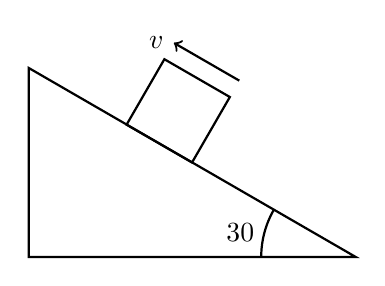
\begin{tikzpicture}[scale=1.2]
          \begin{scope}[thick]
            \draw(0,0)--(-3.46,0)--(-3.46,2)--cycle;
            \draw[thick](-1,0) arc(180:150:1) node[midway,left]{\ang{30}};
            \begin{scope}[rotate=-30]
              \draw(-2,0) rectangle(-2.8,.8);
              \draw[->](-2,1)--(-2.8,1)node[left]{$v$};
            \end{scope}
          \end{scope}
        \end{tikzpicture}
      \end{center}
    }

    \question Which of the following free body diagrams best represents the
    forces acting on the block as it slides up the plane?
    \begin{choices}
      \choice
      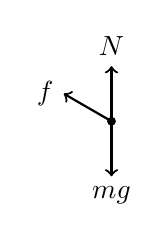
\begin{tikzpicture}[scale=.7]
        \fill[black](0,0) circle(.08);
        \draw[thick,->](0,0)--(0,1) node[above]{$\mb{N}$};
        \draw[thick,->](0,0)--(0,-1)node[below]{$m\mb{g}$};
        \draw[thick,->,rotate=60](0,0)--(0,1)node[left]{$\mb{f}$};
      \end{tikzpicture}
      \choice
      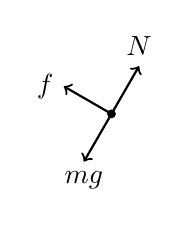
\begin{tikzpicture}[scale=.7]
        \fill[black](0,0) circle(.08);
        \draw[thick,->,rotate=-30](0,0)--(0,1)node[above]{$\mb{N}$};
        \draw[thick,->,rotate=-30](0,0)--(0,-1)node[below]{$m\mb{g}$};
        \draw[thick,->,rotate=60](0,0)--(0,1)node[left]{$\mb{f}$};
      \end{tikzpicture}
      \choice
      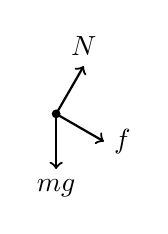
\begin{tikzpicture}[scale=.7]
        \fill[black](0,0) circle(.08);
        \draw[thick,->,rotate=-30](0,0)--(0,1)node[above]{$\mb{N}$};
        \draw[thick,->](0,0)--(0,-1)node[below]{$m\mb{g}$};
        \draw[thick,->,rotate=60](0,0)--(0,-1)node[right]{$\mb{f}$};
      \end{tikzpicture}
      \choice
      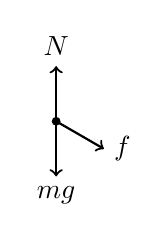
\begin{tikzpicture}[scale=.7]
        \fill[black](0,0) circle(.08);
        \draw[thick,->](0,0)--(0,1)node[above]{$\mb{N}$};
        \draw[thick,->](0,0)--(0,-1)node[below]{$m\mb{g}$};
        \draw[thick,->,rotate=60](0,0)--(0,-1)node[right]{$\mb{f}$};
      \end{tikzpicture}
      \choice
      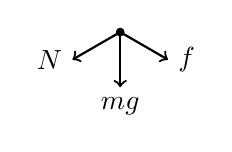
\begin{tikzpicture}[scale=.7]
        \fill[black](0,0) circle(.08);
        \draw[thick,->,rotate=120](0,0)--(0,1)node[left]{$\mb{N}$};
        \draw[thick,->](0,0)--(0,-1)node[below]{$m\mb{g}$};
        \draw[thick,->,rotate=60](0,0)--(0,-1)node[right]{$\mb{f}$};
      \end{tikzpicture}
    \end{choices}
    \label{fbds}
    
  \item The magnitude of the frictional force $f$ between the block and the
    plane is most nearly
    \begin{choices}
      \choice\SI1{\newton}
      \choice\SI2{\newton}
      \choice\SI3{\newton}
      \choice\SI4{\newton}
      \choice\SI5{\newton}
    \end{choices}
    \label{fk}

    \fullwidth{
      \textbf{Questions \ref{plane1}--\ref{plane2}}

      A \SI{10}{\newton} block sits atop an inclined plane in the shape of a
      right triangle of sides \SI{3}{\metre}, \SI{4}{\metre}, and
      \SI{5}{\metre}, as shown. The block is allowed to slide down the plane
      with negligible friction.
      \begin{center}
        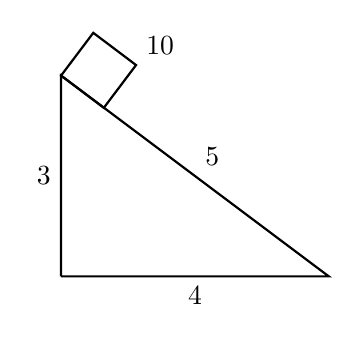
\begin{tikzpicture}[scale=.85]
          \begin{scope}[thick]
            \draw(0,0)--(4,0) node[midway,below]{\SI{4}{\metre}}
            --(0,3) node[midway,above right]{\SI{5}{\metre}}
            --(0,0) node[midway,left]{\SI{3}{\metre}};
            \draw[rotate around={-37:(0,3)}](0,3) rectangle(.8,3.8)
            node[above right]{\SI{10}{\newton}};
          \end{scope}
        \end{tikzpicture}
      \end{center}
    }
    
    \question The acceleration of the block is most nearly
    \begin{choices}
      \choice\SI2{\metre\per\second\squared}
      \choice\SI4{\metre\per\second\squared}
      \choice\SI6{\metre\per\second\squared}
      \choice\SI{10}{\metre\per\second\squared}
      \choice\SI{12}{\metre\per\second\squared}
    \end{choices}
    \label{plane1}
    
    \question The normal force exerted on the block by the plane is most nearly
    \begin{choices}
      \choice\SI{2}{\newton}
      \choice\SI{4}{\newton}
      \choice\SI{6}{\newton}
      \choice\SI{8}{\newton}
      \choice\SI{10}{\newton}
    \end{choices}
    \label{plane2}
   
    \question A constant force acts on a particle in such a way that the
    direction of the force is always perpendicular to its velocity. Which of the
    following is true of the particle's motion?
    \begin{choices}
      \choice The acceleration of the particle is increasing
      \choice The acceleration of the particle is decreasing.
      \choice The speed of the particle is increasing.
      \choice The speed of the particle is constant.
      \choice The speed of the particle is decreasing.
    \end{enumerate}
    \vspace{.7in}

    \fullwidth{
      \textbf{Questions \ref{stacked1}--\ref{stacked2}}\\
      A block of mass \SI{2}{\kilo\gram} rests on top of a larger block of mass
      \SI{4}{\kilo\gram}. The larger block slides without friction on a table,
      but the surface between the two blocks is not frictionless. The
      coefficient of friction between the two blocks is $0.2$. A horizontal
      force $\mb{F}$ is applied to the \SI{4}{\kilo\gram} mass.
      \begin{center}
        \begin{tikzpicture}[scale=.95]
          \fill[pattern=north east lines] (3,0) rectangle(9,-.3);
          \draw[thick] (3,0)--(9,0);
          \draw[thick](5,1) rectangle(6,2) node[midway]{\SI2{\kilo\gram}};
          \draw[thick](4,0) rectangle(7,1) node[midway]{\SI4{\kilo\gram}};
          \draw[thick,->](7,.5)--(8,.5) node[right]{$\mb{F}$};
        \end{tikzpicture}
      \end{center}
    }

    \question What is the maximum force that can be applied such that there is
    no relative motion between the two blocks?
    \begin{choices}
      \choice zero
      \choice \SI{1}{\newton}
      \choice \SI{2}{\newton}
      \choice \SI{4}{\newton}
      \choice \SI{12}{\newton}
    \end{choices}
    \label{stacked1}
    
    \question What is the acceleration of the \SI2{\kilo\gram} block relative
    to the \SI4{\kilo\gram} block if a force is applied to the 4-kg block that
    causes the \SI4{\kilo\gram} block to accelerate at
    \SI3{\metre\per\second\squared} to the right?
    \begin{choices}
      \choice\SI1{\metre\per\second\squared} to the right
      \choice\SI1{\metre\per\second\squared} to the left
      \choice\SI2{\metre\per\second\squared} to the right
      \choice\SI2{\metre\per\second\squared} to the left
      \choice zero
    \end{choices}
    \label{stacked2}
  \end{questions}
\end{multicols*}
\newpage

\genfreetitle{C}{DYNAMICS}{5}

\genfreedirections

\begin{center}
  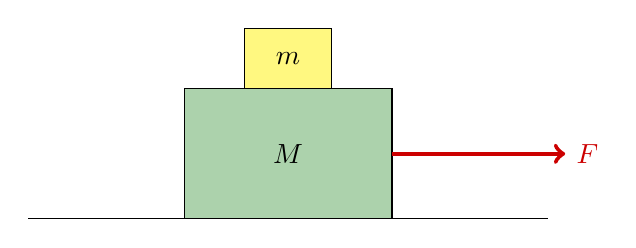
\begin{tikzpicture}[scale=1.1]
    \draw (0,0)--(6,0);
    \draw[fill=green!30!gray!50]
    (1.8,0)rectangle(4.2,1.5) node[midway,black]{$M$};
    \draw[fill=yellow!50](2.5,1.5)rectangle(3.5,2.2)
    node[midway,black]{$m$};
    \draw[ultra thick,red!80!black,->](4.2,.75)--(6.2,.75)
    node[right]{$\mb{F}$};
  \end{tikzpicture}
\end{center}
\begin{questions}
  \question A block with mass $m$ sits on a block of mass $M$ that is resting
  on a frictionless table, as shown below. The coefficient of friction between
  the blocks are $\mu_s=0.30$ and $\mu_k=0.20$.
  \begin{parts}
    \part What is the maximum force $\mb{F}$ that can be applied if the block on
    the top is not to slide on the block on the bottom.
    
    \part If $\mb{F}$ is half this value, find the acceleration of each block
    and the force of friction acting on each block.
    
    \part If $\mb{F}$ is twice the value found in (a), find the acceleration of
    each block.
  \end{parts}
  \newpage
  
%\item A \SI{2.}{\kilo\gram} body rests on a smooth wedge that has an inclination
%  of \ang{60} and an acceleration $\mb{a}$ to the right such that the mass
%  remains stationary relative to the wedge.
%  \begin{enumerate}
%  \item Find acceleration $\mb{a}$.
%  \item What would happen if the wedge were given a greater acceleration?
%    Explain.
%  \end{enumerate}
%  \begin{tikzpicture}[scale=2.1]
%    \draw[ultra thick,green!40!black,->](.5,.6)--(1.7,.6)
%    node[right,black]{$\mb{a}$};
%    \draw(-1,0)--(2,0);
%    \draw[fill=blue!50!gray!50](0,0)--(0,1.7)--(1,0)--cycle;
%    \draw[->](.7,0) arc(180:120:.3) node[midway,left]{\ang{60}};
%    \begin{scope}[rotate around={-59.5:(1,0)}]
%      \draw[fill=red!50!gray!50](0,0) rectangle(-.5,.5)
%      node[midway,black]{\SI{2.}{kg}};
%    \end{scope}
%  \end{tikzpicture}
%  \newpage
%  
%\item A pick-up truck with two stacked crates in the truck bed brakes quickly.
%  The crate on the bottom just barely stays put on the bed of the truck. Does
%  the top crate stay put or does it fall off? The top crate has a mass of
%  \SI{27}{\kilo\gram} and the mass of the bottom crate is \SI{22}{\kilo\gram}.
%  The coefficient of static friction between the bottom crate and the truck is
%  $0.42$, and the coefficient of kinetic friction for that surface is $0.35$.
%  The coefficient of static friction between the crate is $0.40$, and the
%  coefficient of kinetic friction is $0.32$.
%  \vspace{2in}
%  \newpage

  % THIS IS TAKEN FROM THE 2013 AP PHYSICS C FREE-RESPONSE QUESTION MECH 2
  \fullwidth{
    \begin{center}
      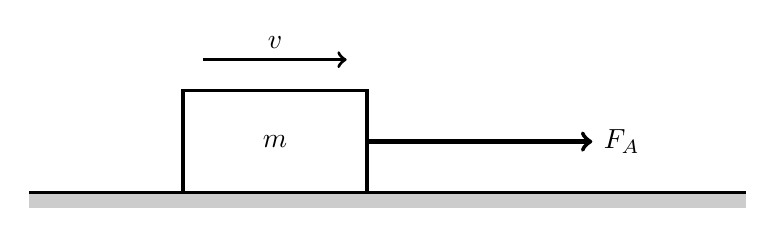
\begin{tikzpicture}[scale=1.3]
        \fill[gray!40](-1.5,-.15) rectangle(5.5,0);
        \begin{scope}[very thick]
          \draw(-1.5,0)--(5.5,0);
        \draw(0,0) rectangle(1.8,1) node[midway]{$m$};
        \draw[->](.2,1.3)--(1.6,1.3) node[midway,above]{$v$};
        \end{scope}
        \draw[ultra thick,->](1.8,.5)--(4,.5) node[right]{$F_A$};
      \end{tikzpicture}
    \end{center}
  }
  
  \question A box of mass $m$ initially at rest is acted upon by a constant
  applied force of magnitude $F_A$, as shown in the figure above. The friction
  between the box and the horizontal surface can be assumed to be negligible,
  but the box is subject to a drag force of magnitude $k\varv$ where $\varv$ is
  the speed of the box and $k$ is a positive constant. Express all your answers
  in terms of the given quantities and fundamental constants, as appropriate.
  \begin{parts}
    \part The dot below represents the box. Draw and label the forces (not
    components) that act on the box.
    \vspace{.5in}
    \begin{center}
      {\tikz\fill(0,0) circle(.2);}
    \end{center}
    \vspace{.5in}

    \part Write, but do not solve, a differential equation that could be used to
    determine the speed $\varv$ of the box as a function of time $t$. If you
    need to draw anything other than what you have shown in part (a) to assist
    in your solution, use the space below. Do NOT add anything to the figure in
    part (a).
    
    \part Determine the magnitude of the terminal velocity of the box.
    
    \part Use the differential equation from part (b) to derive the equation for
    the speed $\varv$ of the box as a function of time $t$. Assume that
    $\varv=0$ at time $t=0$.
    
    \part On the axes below, sketch a graph of the speed $\varv$ of the box as a
    function of time $t$. Explicitly label any intercepts, asymptotes, maxima,
    or minima with numerical values or algebraic expressions, as appropriate.
    \begin{center}
      \begin{tikzpicture}
        \draw[very thick,->](0,0)--(4,0)
        node[pos=0,left]{$O$} node[right]{$t$};
        \draw[very thick,->](0,-3)--(0,3)node[above]{$\varv$};
      \end{tikzpicture}
    \end{center}
  \end{parts}
  \newpage
  
  % THIS IS TAKEN FROM THE 2011 AP PHYSICS C FREE-RESPONSE QUESTION MECH 2
  \fullwidth{
    \cpic{.5}{amusement}
  }
  
  \question An amusement park ride features a passenger compartment of mass $M$
  that is released from rest at point $A$, as shown in the figure above, and
  moves along a track to point $E$. The compartment is in free fall between
  points $A$ and $B$, which are a distance of $3R/4$ apart, then moves along
  the circular arc of radius $R$ between points $B$ and $D$. Assume the track is
  frictionless from point $A$ to point $D$ and the dimensions of the passenger
  compartment are negligible compared to $R$.
  \begin{parts}
    \part On the dot below that represents the passenger compartment, draw and
    label the forces (not components) that act on the passenger compartment
    when it is at point $C$, which is at an angle $\theta$ from point $B$.
    \begin{center}
      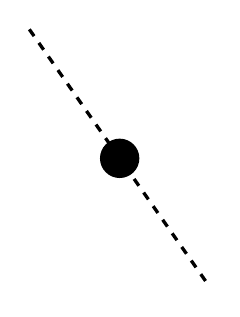
\begin{tikzpicture}
        \fill(0,0) circle(.25);
        \draw[rotate=35,dashed,very thick](0,2)--(0,-2);
      \end{tikzpicture}
    \end{center}
    
    \part In terms of $\theta$ and the magnitudes of the forces drawn in part
    (a), determine an expression for the magnitude of the centripetal force
    acting on the compartment at point $C$. If you need to draw anything
    besides what you have shown in part (a) to assist in your solution, use the
    space below. Do NOT add anything to the figure in part (a).

    \part Derive an expression for the speed $\varv_D$ of the passenger
    compartment as it reaches point $D$ in terms of $M$, $R$, and fundamental
    constants, as appropriate.
  
    \uplevel{
      A force acts on the compartment between points $D$ and $E$ and brings it
      to rest at point $E$.
    }
    
    \part If the compartment is brought to rest by friction, calculate the
    numerical value of the coefficient of friction $\mu$ between the
    compartment and the track.
    
    \uplevel{
      Now consider the case in which there is no friction between the
      compartment and the track, but instead the compartment is brought to rest
      by a braking force $-k\mb{v}$, where $k$ is a constant and $\mb{v}$ is the
      velocity of the compartment. Express all algebraic answers to the
      following in terms of $M$, $R$, $k$, $v_D$, and fundamental constants, as
      appropriate.
    }

    \part Write, but do NOT solve, the differential equation for $\varv(t)$.
    \label{diffeq}
    
    \part Solve the differential equation you wrote in part (\ref{diffeq}).
    
    \part On the axes below, sketch a graph of the magnitude of the
    acceleration of the compartment as a function of time. On the axes,
    explicitly label any intercepts, asymptotes, maxima, or minima with
    numerical values or algebraic expressions, as appropriate.
    \begin{center}
      \begin{tikzpicture}[scale=1.2]
        \begin{scope}[very thick,->]
          \draw(0,0)--(7,0) node[midway,below]{Time};
          \draw(0,0)--(0,3) node[above]{Magnitude of Acceleration};
        \end{scope}
      \end{tikzpicture}
    \end{center}
  \end{parts}
\end{questions}
\end{document}
